\documentclass{article}\usepackage[]{graphicx}\usepackage[]{color}
% maxwidth is the original width if it is less than linewidth
% otherwise use linewidth (to make sure the graphics do not exceed the margin)
\makeatletter
\def\maxwidth{ %
  \ifdim\Gin@nat@width>\linewidth
    \linewidth
  \else
    \Gin@nat@width
  \fi
}
\makeatother

\definecolor{fgcolor}{rgb}{0.345, 0.345, 0.345}
\newcommand{\hlnum}[1]{\textcolor[rgb]{0.686,0.059,0.569}{#1}}%
\newcommand{\hlstr}[1]{\textcolor[rgb]{0.192,0.494,0.8}{#1}}%
\newcommand{\hlcom}[1]{\textcolor[rgb]{0.678,0.584,0.686}{\textit{#1}}}%
\newcommand{\hlopt}[1]{\textcolor[rgb]{0,0,0}{#1}}%
\newcommand{\hlstd}[1]{\textcolor[rgb]{0.345,0.345,0.345}{#1}}%
\newcommand{\hlkwa}[1]{\textcolor[rgb]{0.161,0.373,0.58}{\textbf{#1}}}%
\newcommand{\hlkwb}[1]{\textcolor[rgb]{0.69,0.353,0.396}{#1}}%
\newcommand{\hlkwc}[1]{\textcolor[rgb]{0.333,0.667,0.333}{#1}}%
\newcommand{\hlkwd}[1]{\textcolor[rgb]{0.737,0.353,0.396}{\textbf{#1}}}%
\let\hlipl\hlkwb

\usepackage{framed}
\makeatletter
\newenvironment{kframe}{%
 \def\at@end@of@kframe{}%
 \ifinner\ifhmode%
  \def\at@end@of@kframe{\end{minipage}}%
  \begin{minipage}{\columnwidth}%
 \fi\fi%
 \def\FrameCommand##1{\hskip\@totalleftmargin \hskip-\fboxsep
 \colorbox{shadecolor}{##1}\hskip-\fboxsep
     % There is no \\@totalrightmargin, so:
     \hskip-\linewidth \hskip-\@totalleftmargin \hskip\columnwidth}%
 \MakeFramed {\advance\hsize-\width
   \@totalleftmargin\z@ \linewidth\hsize
   \@setminipage}}%
 {\par\unskip\endMakeFramed%
 \at@end@of@kframe}
\makeatother

\definecolor{shadecolor}{rgb}{.97, .97, .97}
\definecolor{messagecolor}{rgb}{0, 0, 0}
\definecolor{warningcolor}{rgb}{1, 0, 1}
\definecolor{errorcolor}{rgb}{1, 0, 0}
\newenvironment{knitrout}{}{} % an empty environment to be redefined in TeX

\usepackage{alltt}[11pt]
%Required: You must have these
\usepackage{graphicx}
\usepackage{tabularx}
\usepackage{natbib}

\usepackage{array}
\usepackage{amsmath}
%\usepackage[backend=bibtex]{biblatex}
\setkeys{Gin}{width=0.8\textwidth}
%\setlength{\captionmargin}{30pt}
\setlength{\abovecaptionskip}{10pt}
\setlength{\belowcaptionskip}{10pt}
\topmargin -1.5cm 
\oddsidemargin -0.04cm 
\evensidemargin -0.04cm 
\textwidth 16.59cm
\textheight 23.94cm 
\parskip 7.2pt 
\renewcommand{\baselinestretch}{1.2} 	
\parindent 0pt


\bibliographystyle{..//..//refs/styles/besjournals.bst}
%\usepackage{xr-hyper}
\usepackage{hyperref}
\title{Aridity drive hysteranthous flowering in the American Plums (\textit{Prunus} sect. \textit{prunocerasus})}
\IfFileExists{upquote.sty}{\usepackage{upquote}}{}
\begin{document}
\maketitle


\section*{Introduction}

\noindent Woody perennials have a unique ability among plants to seasonally begin reproduction prior to vegetative growth This flowering-first phenological sequence known as hysteranthy, proteranthy or precocious flowering is particularly common in temperate forests around the globe \citep{Rathcke_1985}. A number of studies suggest that this flower-leaf sequences (FLSs) are under selection, and that flowering first has functional significance \citep{Gougherty2018,Buonaiuto2020,Guo2014}.

\noindent The most common, and well-tested explanation for the evolution of hysteranthy in temperate forest is that is that it is adaptive for wind-pollination as leafless canopies increase wind speeds for pollen transport and reduce the likelihood of pollen interception on vegetation \citep{Whitehead1969,Niklas1985}. However, this hypothesis fails to address the prevalence of hysteranthous taxa that are biotically-pollinated. Approximately 30\% of species of Eastern temperate forests of North America flower before leafing out, and of those, approximately 20\% are biotically pollinated  \citep{Buonaiuto2020}. Despite the pervasiveness of this phenological syndrome, direct tests of the function of hysteranthy in biotically pollinated taxa are exceedingly rare for temperate forest species.

However, looking to other biomes in which hysteranthous flowering is also common shed offers important insights regarding the function of hysteranthyin temperate, biotically-pollinated taxa. In the dry-deciduous tropics of South and Central America, flowering during the leafless period is also common \citep{Rathcke_1985,Franklin2016}, flowering is associated with a recovery in plant water status due to leaf drop \citep{Borchert1983,Reich1984}. By temporally separating leaf and flower activity, woody plants can partition the hydraulic demand across the season, alleviating water stress \citep{Gougherty2018,Franklin2016}. These physiological observations suggest that hysteranthous flowering may be an adaptation to arid environments.

While it is unclear whether this hydraulic demand hypothesis (also known as water dynamic hypothesis \citep{Gougherty2018} or water limitation hypothesis \citep{Buonaiuto2020}) is relevant in the temperate zone where forests are rarely water-limited  in the early season during which flowering and leafing occur \citep{Polgar2011}, the hypothesis makes several predictions that can be tested to evaluate whether hysteranthy serves to increase aridity tolerance in temperate flora:
\begin{enumerate}
\item Hysteranthous taxa should be found in dryer habitats compared to closely relate, non-hysteranthous species.
\item Hysteranthy may be linked to other reproductive traits associated with dry environments such as reduced flower and fruit size \citep{Herrera:2009aa,Liu:2013ua}.
%\item Additionally, flower-leaf sequences can be highly variable within individuals across time \citep{}, and if hysteranthy contributes to aridity tolerance, climate variability may be positively correlated with variability in hysteranthy.
\end{enumerate}
%\noindent Yet, based on decades of natural history accounts of hysteranthous species around th globe, we present two hypotheses regarding the function of hysteranthy in biotically-pollinated taxa. Each hypothesis makes logical predictions about how hysteranthous flowering should other plant traits should co-vary, and these hypotheses and their predictions can be used to guide further inquiry into the adaptive significance of hysteranthy.

%The \textbf{water dynamics hypothesis} suggests that hysteranthy is an adaptation to arid environments, allowing for plant to partition the hydraulic demand of hydrated flowers and transpiring leaves across the growing season \citep{}. If this is the case, this hypothesis predicts that hysteranthous species should be more commonly found in dry environments.  

%The \textbf{pollinator visibility hypothesis} suggests that hysteranthy is an adaptation to attract visually-foraging pollinators \citep{}. If this is the case, this hypothesis predicts that hysteranthous species may invest less in other floral traits for pollinator attraction such as size of floral display or chemical attraction. 

%\noindent Still others have suggested that hysteranthy is simply the by-product of selection for early flowering \citep{},and that variation in flower-leaf sequences among species is driven by developmental, physical or phylogenetic constraints than adaptive selection \citep{}. However, even this null hypothesis make testable predictions. If this is the case, hysteranthy should co-vary with other early-flowering associated traits like long fruit development periods or large fruit sizes \citep{} and the phylogenetic signal for hysteranthy should be strong.

\noindent With mounting evidence anthropogenic cliamte change is both driving shifts in flower-leaf sequences \citep{Ma2020:aa} and changing geographic patterns of water availability \citep{}  understanding the functional significance of hysteranthy is vital to forecasting the demography and performance of forest communities in an era of global climate change. However, there are two major methodological challenges to testing these hypotheses:

\noindent First, characteristics like aridity tolerance, are the emergent product of a suite of biological traits \citep{Simova:2017vk}. Thus, when analyzing selective drivers of any particular trait at large taxonomic scales, unmeasured trait differences may obscure the estimated effects of the trait of interest, biasing results. %For example, hysteranthy may contribute significantly to differences in aridity tolerance between two species with similar root architecture, leaf characteristics and xylem anatomy, but matter much less when comparing deep rooted species to shallow rooted ones. 
This is a common problem in trait-based ecology, and one of the most promising solutions for understanding the functional significance of hysteranthy in woody plants is through character deconstruction \citep{Terribile2009}; comparing flower-leaf sequences variation for only a subset of taxa of shared phylogenetic and morphological character.   

\noindent A second challenge for robust testing of hysteranthy hypotheses is that most characterizations of flower-leaf phenological sequences are based on expert-opinion verbal descriptions(e.g. ``flowers before leaves" or ``flower before/with leaves"), which make comparisons across taxa, time and space difficult sensitive to observer bias (see, \citep{Buonaiuto2020}). 

\noindent This problem can be overcome by adopting standardized quantitative measures of plant phenology for observational studies and applying them to historic data records. Herbarium records are an excellent source of data that can be leveraged for quantitative phenological measurements \citep{Willis2017}, but have not be used widely to investigate variability of flower-leaf sequences variation among and within species.

\noindent In this study, %we begin by combining a large data set of occurrence records with published descriptions of flower-leaf sequences and plant traits for North American species in the genus \textit{Prunus} to test the predicted trait associations of the major hysteranthy hypotheses at the genus level. We then shift our focus to one sub-clade within the genus, the American plums, (subsp \textit{Prunus}, sect. \textit{Prunocerasus}. 
we used herbaria records to to quantify flower-leaf sequences both within and among species in the American plums, (subsp \textit{Prunus}, sect. \textit{Prunocerasus}. We then evaluated the association between hysteranthy and several ecological and morphological traits to test the prediction of the hydraulic demand hypothesis of hysteranthy. Our findings both clarify the hypothesized function of flower-leaf sequence variation in biotically pollinated taxa and offer insights into how flower-leaf sequences may impact species distrubutions as cliamte continues to change.


%<<>>=
%mich.data<-read.csv("..//..//sub_projs/MTSV_USFS/michdata_final.csv")
%table(mich.data$pro2,mich.data$Pollination)

%table(mich.data$pro)
%42/147
%table(mich.data$pro2)
%82/147

@

%Generally speaking, hysteranthy is unique and common in temperate forest. Seems functionial. The most common, and well tested, explaination is that is hysteranthy evolved for wind-pollination. However that doesn't explain its prevalence in biotically pollinated taxa. Quote some statistic based new phyt paper. Tests of the function on hysteranthy in biotically pollinated taxa are exceedingly rare in the literature,, but may be critial for predicting species responses to global change.

%While direct tests are limited, investegation of hysteranthy beneifit from a rich theoretical literature and several hypotheses have emerge.

%Review them briefly and make predictions
%\begin{enumerate}
%\item Drought adaptation: (could be plastic or selected) aridity in range
%\item insect visaibility: floral morphology
%\item Null functionality early flowering. Fruit size or phenology
%\item Phylogeny may also matter
%\end{enumerate}

%While each hypothesis generates testible predictions there are several methodological challenges.
%\begin{enumerate}
%\item Unmeasured species difference compensate for measure traits
%\item data quality based on expert opinion
%\end{enumerate}

%These issues could be over come with:
%\begin{enumerate}
%\item character deconstruction
%\item detailed quantitative measurements of flower leaf sequence phenology
%\end{enumerate}

%We do this:
%\begin{enumerate}
%\item Coarse analyses of the flower-leaf sequences of North American \textit{Prunus} species and their hypothesis relevant traits based on published data
%\item Higher resolution inquiry of the fLower-leaf sequences and associated character traits based on our own measurements from a century worth of herbaria samples on a section of the Prunus subgenus Prunocerasus the American plums
%\end{enumerate}

\section*{Methods}
\subsection{Study system}
%\noindent The genus \texit{Prunus} comprises approximately 200 species distributed across the globe \citep{}. Of 40-50 species native to or naturalized in North America, \textit{Prunus}species display the full spectrum of variation in flower-leaf sequences \citep{} and show marked inter-specific variation in habitat requirements and functional traits making them an ideal system in which to investigate the inter-relationship between hysteranthy and traits predicted by the two major hysteranthy hypotheses.

\noindent The genus \texit{Prunus} comprises approximately 200 species distributed across the globe \citep{Chin:2014wu}, Within the genus, The American plums (\textit{Prunus} subsp. \textit{Prunus} sect. \textit{Prunocerasus}) offer potential for a higher resolution investigation of drivers of hysteranthous flowering. Like the genus at large, the 16 species that make up the section are distributed across North America and show pronounced inter-specific variation in flower-leaf sequences. While within the larger genus species can be separated into three distinct morphological clades by inflorescence architecture (solitary, corymbose or racemose) all members of the section have solitary inflorescences \citep{Shaw:2004aa} allowing for  refined character deconstruction. Species in this section are well represented in herbaria records (Fig. \ref{fig:mappy}), making them a tractable group to measure and assess intra-specific variation in flower-leaf sequences as well as other ecological and morphological characteristics related to the hysteranthy hypotheses described above. 

%\subsection{Genus level analyses}
%To assess the relationship between hysteranthous flowering and morphological and ecological traits related to the hysteranthous hypothesis we obtained flower-leaf sequence descriptions and mean estimates of flower petal length, flowers per inflorescence, and fruit diameter for 44 \textit{Prunus} species from the Flora of North America. As a measure of aridity tolerance, we obtained the coordinates of herbaria occurrence records of all 44 species from the Consortium of Midwest Herbaria digital Archeives (n=23,272). For records that we not geo-referenced was assigned coordinates to the county centroid in which the specimen was observed. We than extracted the average value of Palmer Modified Drought Index from at each local from the North America Drought Atlas \citep{} averaging these values across all occurrence per species for a coarse estimate of species level aridity tolerance. 

%\noindent To assess the relationship between inter-specific flower-leaf sequences variation and the traits predicted by the two hysteranthy hypotheses we fit a Bayesian ordinal regression model with each measured trait (mean pdsi, fruit diameter, flower petal length and flowers per inflorescence) as main effects. In this model, we included an interaction term between flower petal length and number of flowers per inflorescence to account for a well established trade off between these two elements of floral displays \citep{}.
%To be able to directly compare the effects of the of our multi-scale trait and environmental variables, we standardized all predictors in the model through z-scoring \citep{}. We fit all models using the R package ``brms" \citep{Burkner2018} on four chains with 4000 iterations and a 3000 iteration warm up for a total of 4000 posterior draws for each parameter. We used weakly informative priors, and assessed model performance through ensuring $\hat{R}$s were between 1 and 1.01 and bulk and tail effective sample sizes were high (1800-2800 for most parameters, but as low as  800-900 for some).

\subsection{Quantifying flower-leaf sequence variation}
We obtained digital herbarium specimens for all member of the section \textit{Prunocerasus} from the Consortium of Midwest Herbaria Database. To quantify the flower-leaf sequence sequence variation within and across species we randomly sample 200 specimens for each species and scored the phenological development of flower and leaves in accordance with using a modified BBCH scale for woody plants \citep{Finn2007}. In total, we evaluated the phenology of 2521 specimens, but only specimens with visible flower were included in this analysis (n=1009). We reconstructed the phylogenetic relationships among species in this group based on the tree topology in \citet{Shaw:2004aa}. Follwing the methods of \citet{Granfen1989} we computed branch lengths for this phylogeny by assigning each node a height and computing the distance between upper and lower nodes using the function compute.brlen() in the R package ``ape" \citep{}.

To quantify FLS variation, we fit an ordinal, hierarchical, Bayesian, phylogenetic mixed model \citep{Garamszegi2014} to assess the likelihood an individual would be at any given vegetative bbch phase given it is flowering. Because we expect that hysteranthous may be more likely to occur earlier in the flowering period and species differ in their flowering periods, we included the day of the observation as a varying slope, main effect in the model and species and phylogeny as random effects. The model is written below:\\

  %Pr(y_i &=1) &= logit^{-1} \alpha_{j0sp[i]} + \alpha_{phylo[i]} + \beta_{day of year}X_1_[_i_] 
  
$logit(P(Y \leq j)) &= \beta_{[j]sp[i]}+ \beta_{[j]sp[i]}+ \beta_{day of year[sp[i]]}*X_1+ \epsilon_{i}$\\
  
   \epsilon_i & \sim N(0,\sigma^2_y) \\ 
   
   where Y is the ordinal outcome (leaf stage) and j is the number of categories (1,2,...6). $P(Y \leq j))$ is the probability of Y less than of equal to a category j&=1,...j&-1.  In this varying slope and intercept model, $\beta_{[j]}$ describes an intercept for each category [1,2,...6], while slope \$beta_{day of year[sp[i]]}$ is constant across categories. 
  
  \noindent The influence of the phylogeny $\alpha_{phylo}$ was modeled as follows:\\
  \alpha_{sp} & \sim N(\mu_{\alpha}, COR[\sigma^2_{phylo}]) \\
  
  \noindent THe $\alpha$ for species effects independent of the phylogeny was modeled as follows:\\
  \alpha_{sp} & \sim N(\mu_{\alpha}, \sigma^2_{species}) \\

 We fit the model in the R package ``brms" \citep{} usinf weakly informative priors, and ran the model on four chains with a warmup of 3,000 iterations and 4,000 sampling iterations for a total of 4,000 sampling iterations. Model fit was assessed with Rhats <1.01 and high effective sample sizes.
 
Because the day of observation strongly influenced the BBCH stage likelihood, quantifying flower-leaf sequences among species was intractable without accounting for this temporal trend. To address this issues, we used our model to predict the likelihood each species would be observed at a given vegetative BBCH stage during flowering at the 0\%, 25\% 50\% and 75\% quartiles of their flowering period. We then developed a flower-leaf sequence index, by assigning a numerical score to each species per seasonal quantile, and summing over the full flowering season. In each seasonal quantile, species received a 1 if more that 25\% of their probability distribution occurred at BBCH 0, and a 0 if not. These values were summed across the season generating an index from 0 (never hysteranthous) to 4 (hysteranthous through late season (Q75)), where 1&= hysteranthous at start of season, 2&= hysteranthous through early season  (Q25) and 3 &= hysteranthous  through mid season (Q50).

\subsection{Evaluating the hydralic demand hypothesis}

To test the predictions of the hydralic demand hypothesis of hysteranthy we obtained data on  petal length, fruit diameter and directly from herbarium specimens and characterized the aridity of the sites specimens were collected from using the Palmer Modified Drought Index.

\noindent For our morphological measurements, we sampled an additional 321 specimens measured the petal length of up to 10 randomly selected petals per specimen (n=2757) using ImageJ image processing software. We also used ImageJ to measure the diameter of fruits on an additional 316 specimens, measuring up to 5 fruit per specimen (n=224).
We computed the average Palmer Modified Drought Index score from 1900-2017 for every \textit{Prunocerasus} specimen in the database (n=2305) from the North America Drought Atlas \citep{Cook2004}.

We than used Bayesian phylogenetic mixed models to test the relationship between flower-leaf sequence index score and each of the variables. In these models, we included species as the random effect and for traits like flower petal length and fruit diameters than included multiple measurements per specimen, we also included specimen ID as an additional random effect. The model structure is written below: 


  y_i &= \alpha_{ind/sp[i]} +\alpha_{phylo[i]} + \beta_{hyst.index}*X_{hyst.index} + \epsilon_i\\
  
  \epsilon_i & \sim N(0,\sigma^2_y) \\ %Check this
  
  \noindent The effect of the phylogeny was model as above and here, the individual effects within species were modeled:\\
  \alpha_{ind/sp} & \sim N(\mu_{\alpha}, \sigma^2_{ind/sp}) \\
  



%\noindent Because our data dependent and independent were collect we employed a sequential modeling approach to first estimate the mean and standard error of the posterior distribution of trait values for each species then model the relationship between these estimate and the likelihood of hysteranthy using Bayesian measurement error models. This approach propagates the error in the initial estimates of trait values into the our final model, yielding a more accurate evaluation than using mean trait values alone \citep{}. For each parameter of interest, we ran Bayesian phylogenetic mixed-effects models with our measured traits as the response variable and species as the random effect. For traits like flower petal length and fruit diameters than included multiple measurements per specimen, we included specimen ID as an additional random effect. The model structure is written below:

%\noindent Then using each of these trait mean estimates as predictors, we modeled their associations with flower leaf sequences OF using a repeat measure phylogenetic mixed ordinal regression in brms \citep{}. Because we found the three predictors of interested to be highly colinear (pariwise correlations >0.5), we ran one regression model per predictor trait to avoid skewing our model inference due to multi-collinearity \citep{MacElreath, Nations}.

%For all models in the sequences,


\section*{Results}
\subsection*{Quantifying flower leaf sequences in the American plums}
We found that strong inter-specific difference in flower leaf sequences in with the American plums, and that patterns were strongly dependent on the day of observations, with observations later in the the flowering season of each species decreasing the likely hood of finding flowers open during early vegetative BBCH phases ($\beta_{doy}$: 0.0278 SE:0.0059, Fig.\ref{}). Based on our flower leaf sequence index, two species (\textit{P. umbellata},\text{P. mexicana}) were likely to be hysteranthous regardless of the time of observation and three species (\textit{P. rivularis},\texit{P. subcordata}, and \textit{P. texana}) were alway most likely to flower after level expansion began (Fig. \ref{Fig.}). All other species displayed intermediate phenotypes with five species mostly likely to hysteranthous at the start of the season (\textit{P. alleghaniensis},\texit{P. americana},\textit{P. hortulana},\textit{P. munsoniana} and \texit{P. nigra}), one species through early season (\textit{P gracilis}) and two species through mid season (\textit{P. angustifolia}, \textit{P. maritima}) (Fig \ref{}).

\subsection*{Evaluating the Hydraulic demand hypothesis}
We found a negative association between flower-leaf sequence index and mean pdsi (), suggesting that species that displayed hysteranthous flowering later into their flowering season were found in dryer locations. 

We found a negative association between flower-leaf sequence index and both  petal length and fruit diameter (X,Y respectively), though the relationship between FLS index and fruit size was much stronger.

We found no relationship between the likelihood of hysteranthy and pdsi.

%\subsection*{Drivers of hysteranthy in\textit{Prunus spp.} of North America}
%Increased likelihood of hysteranthy was associated increasing aridity, flowering and inflorescence size and their interaction. Fruit size had little effect of the likelihood of hysteranthy and at the genus level, the phylogenetic signal in hysteranthy was X suggesting weak to moderate phylogeny structure.


%\subsection*{Drivers of hysteranthy in sect. \textit{Prunocerasus} }
%Within the section \textit{Prunocerasus}, hysteranthy was associated with smaller fruit (). There was no relationship between flower size, fruit phenology, or mean pdsi and the phylogenetic signal of hysteranthy was virtually non-existent within this sub-clade. When we investigated

\section*{Discussion}
We found hysteranthy is associated with drier average conditions. We also found its associated with small flowers and fruits. Support the hypothesis.
We did not find it for the plasticity piece.

Compare this to the relative physiology of flower and frutis.

Observe that two of the three no hysteranthy species are phylogentically and geographically distinct

Talk about how this analysis is outside of the Eastern temperature forests that most have studied. 

Other clades

Make the point that while

%The associations between the likelihood of hysteranthy flower/inflorescence size and aridity between we detected at the genus suggests tacit support for both the insect visibility hypothesis and the water dynamics hypothesis. However we must emphasize that our analysis detected an association between hysteranthous phenology and reduced floral displays, but we cannot empirically identify the evoloutionary mechanisms driving this relationship. While the relationship certainly may indicate a trade-off between the apparent visibility of flowers and investment in the floral structures that is predicted by the insect visibility hypothses, there are numerous other evolutionary or developmental forces that could drive this relationship. For example, species with large inflorescence may not be able to store enough carbohydrates to produce and maintain these structure before leaf emergence, and the relationship we detected could a readily be evidence of a developmental constraint on hysteranthous flowering as evidence of adaptive selection.  Sespite the strong relationship between flower display size and hysteranthy we detected in our study that follows the predicted pattern of insect-visibility hypothesis, we cannot unequivocally assert that hysteranthy is an adaptation for pollinator attraction. What can we say? I think that the relationship suggests this is an avenue to pursue and here is a place we could talk about mechanisnistic experiments.

%\noindent In contrast to the strong associations we detected at the genus level, within the section of \text{Prunocerasus}, fruit size was the only trait significantly associated with increased likelihood of hysteranthy. However, the estimated effect was relatively weak, and the positive relationship between fruit size and FLS catagory (suggestion that hysteranthy is associated with smaller fruit), is counter to the expectation about the relationship between fruit size and flowering time \citep{}.

%\noindent The dissimilarity in the relationships between the likelihood of hysteranthy and predicted traits we observed at the genus and section level could describe a biological phenomenon indicating at what phylogenetic scale the evolution of hysteranthous flowering may be adaptive. Alternatively, because our analyses at the genus and section level leveraged different kinds of phenological and trait data, and differed in their ability to account for intra-specific variation and  measurement error, the differences we observed among taxonomic scales may be a statistical issues rather than a biological one. While we cannot definitively separate the effects of biology and methodology on the outcomes of this study (), following each line of reason provides important paths forward for future studies of hysteranthy flowering and trait-based evolutionary ecology in general.




%At the genus level we identified a strong negative relationship between the likelihood a species is hysteranthous and flower size, inflorescence size and aridity (). Fruit size appeared to have little influence on hysteranthy () and the phylogenetic signal for in the evolution of flower-leaf sequences was weak-moderate (). Phylogenetic structure in flower-leaf sequences was moderate within the genus. By contrast, with in the section of \text{Prunocerasus}, fruit size was the only trait significantly associated with increased likelihood relationship. However, the estimated effect was relatively weak, and the positive relationship between fruit size and FLS catagory (suggestion that hysteranthy is associated with smaller fruit), is counter to the expectation about the relationship between fruit size and flowering time\ \citep{}. Looking at this subclade, the phylogenetic signal for flower-leaf sequence patterns was negligible.

\noindent  


\bibliography{..//..//..//sub_projs/refs/hyst_outline.bib} 




\newpage
\section*{Figures}
    \begin{figure}[h!]
    \centering
 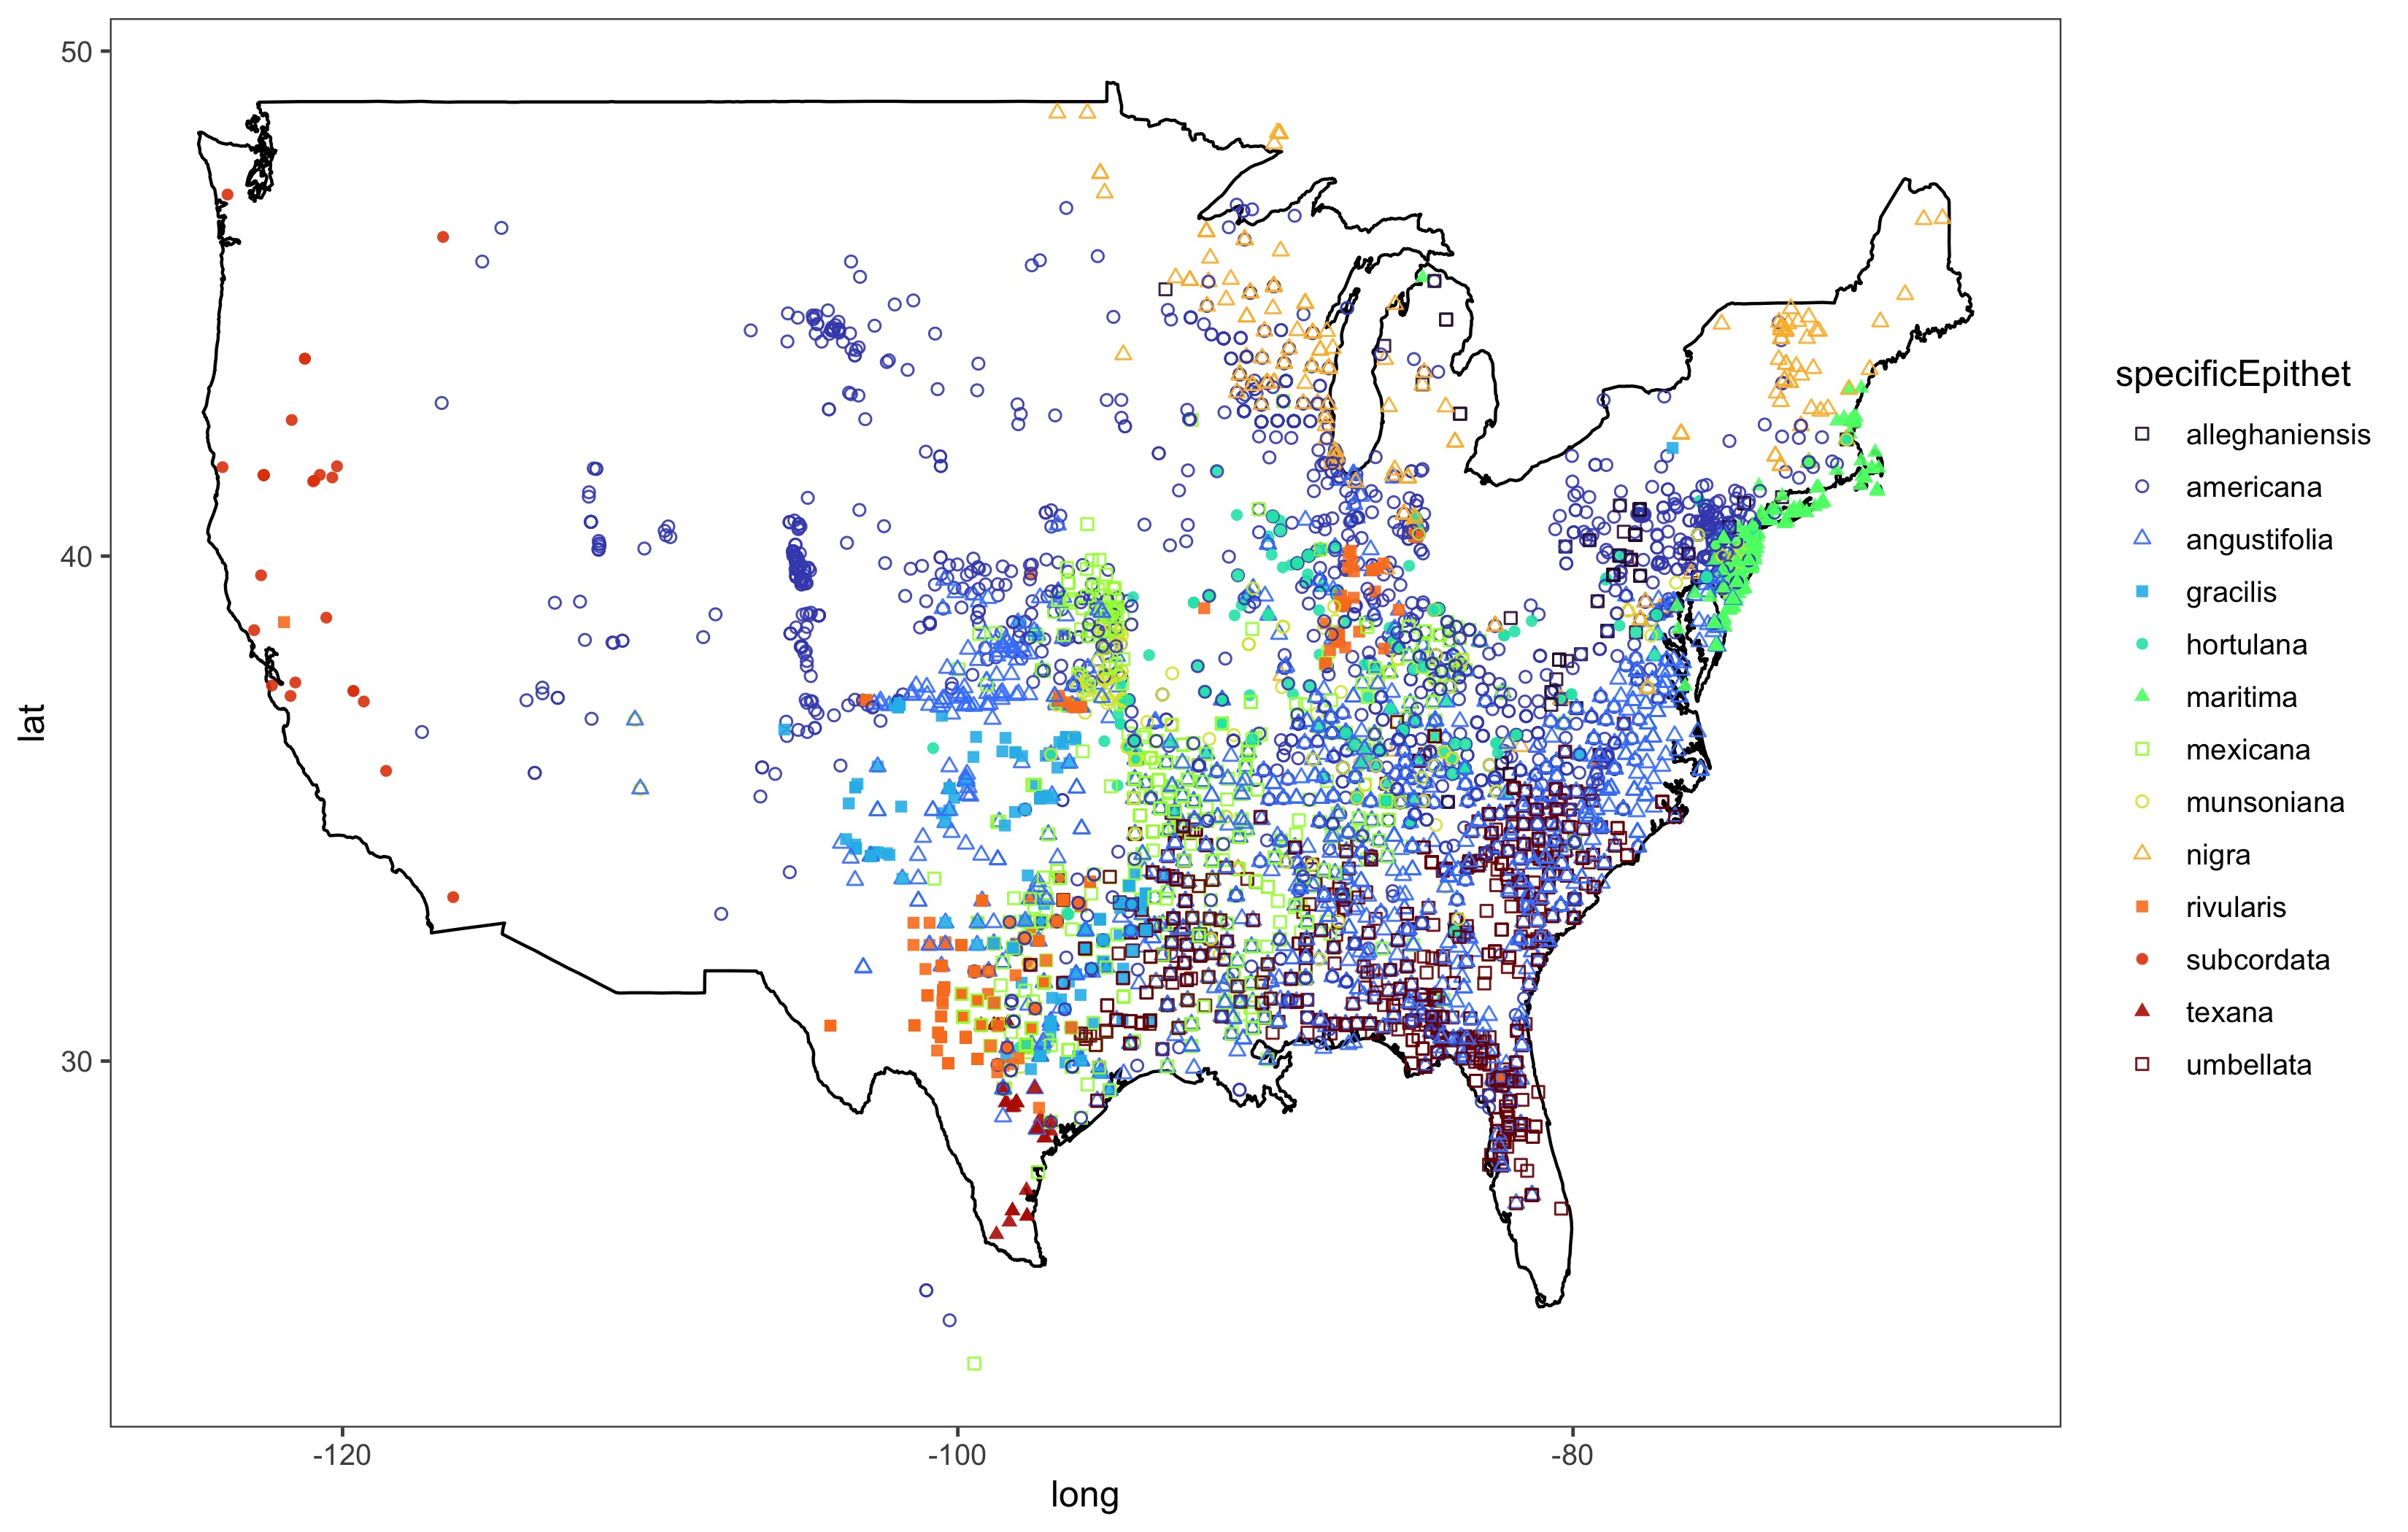
\includegraphics[width=\textwidth]{..//..//Plots/map.jpeg}
    \caption{Map to show where data come from and to point out the two never hysteranthy species are highly endemic}
    \label{fig:mappy}
\end{figure}

%\begin{figure}[h!]
%    \centering
% 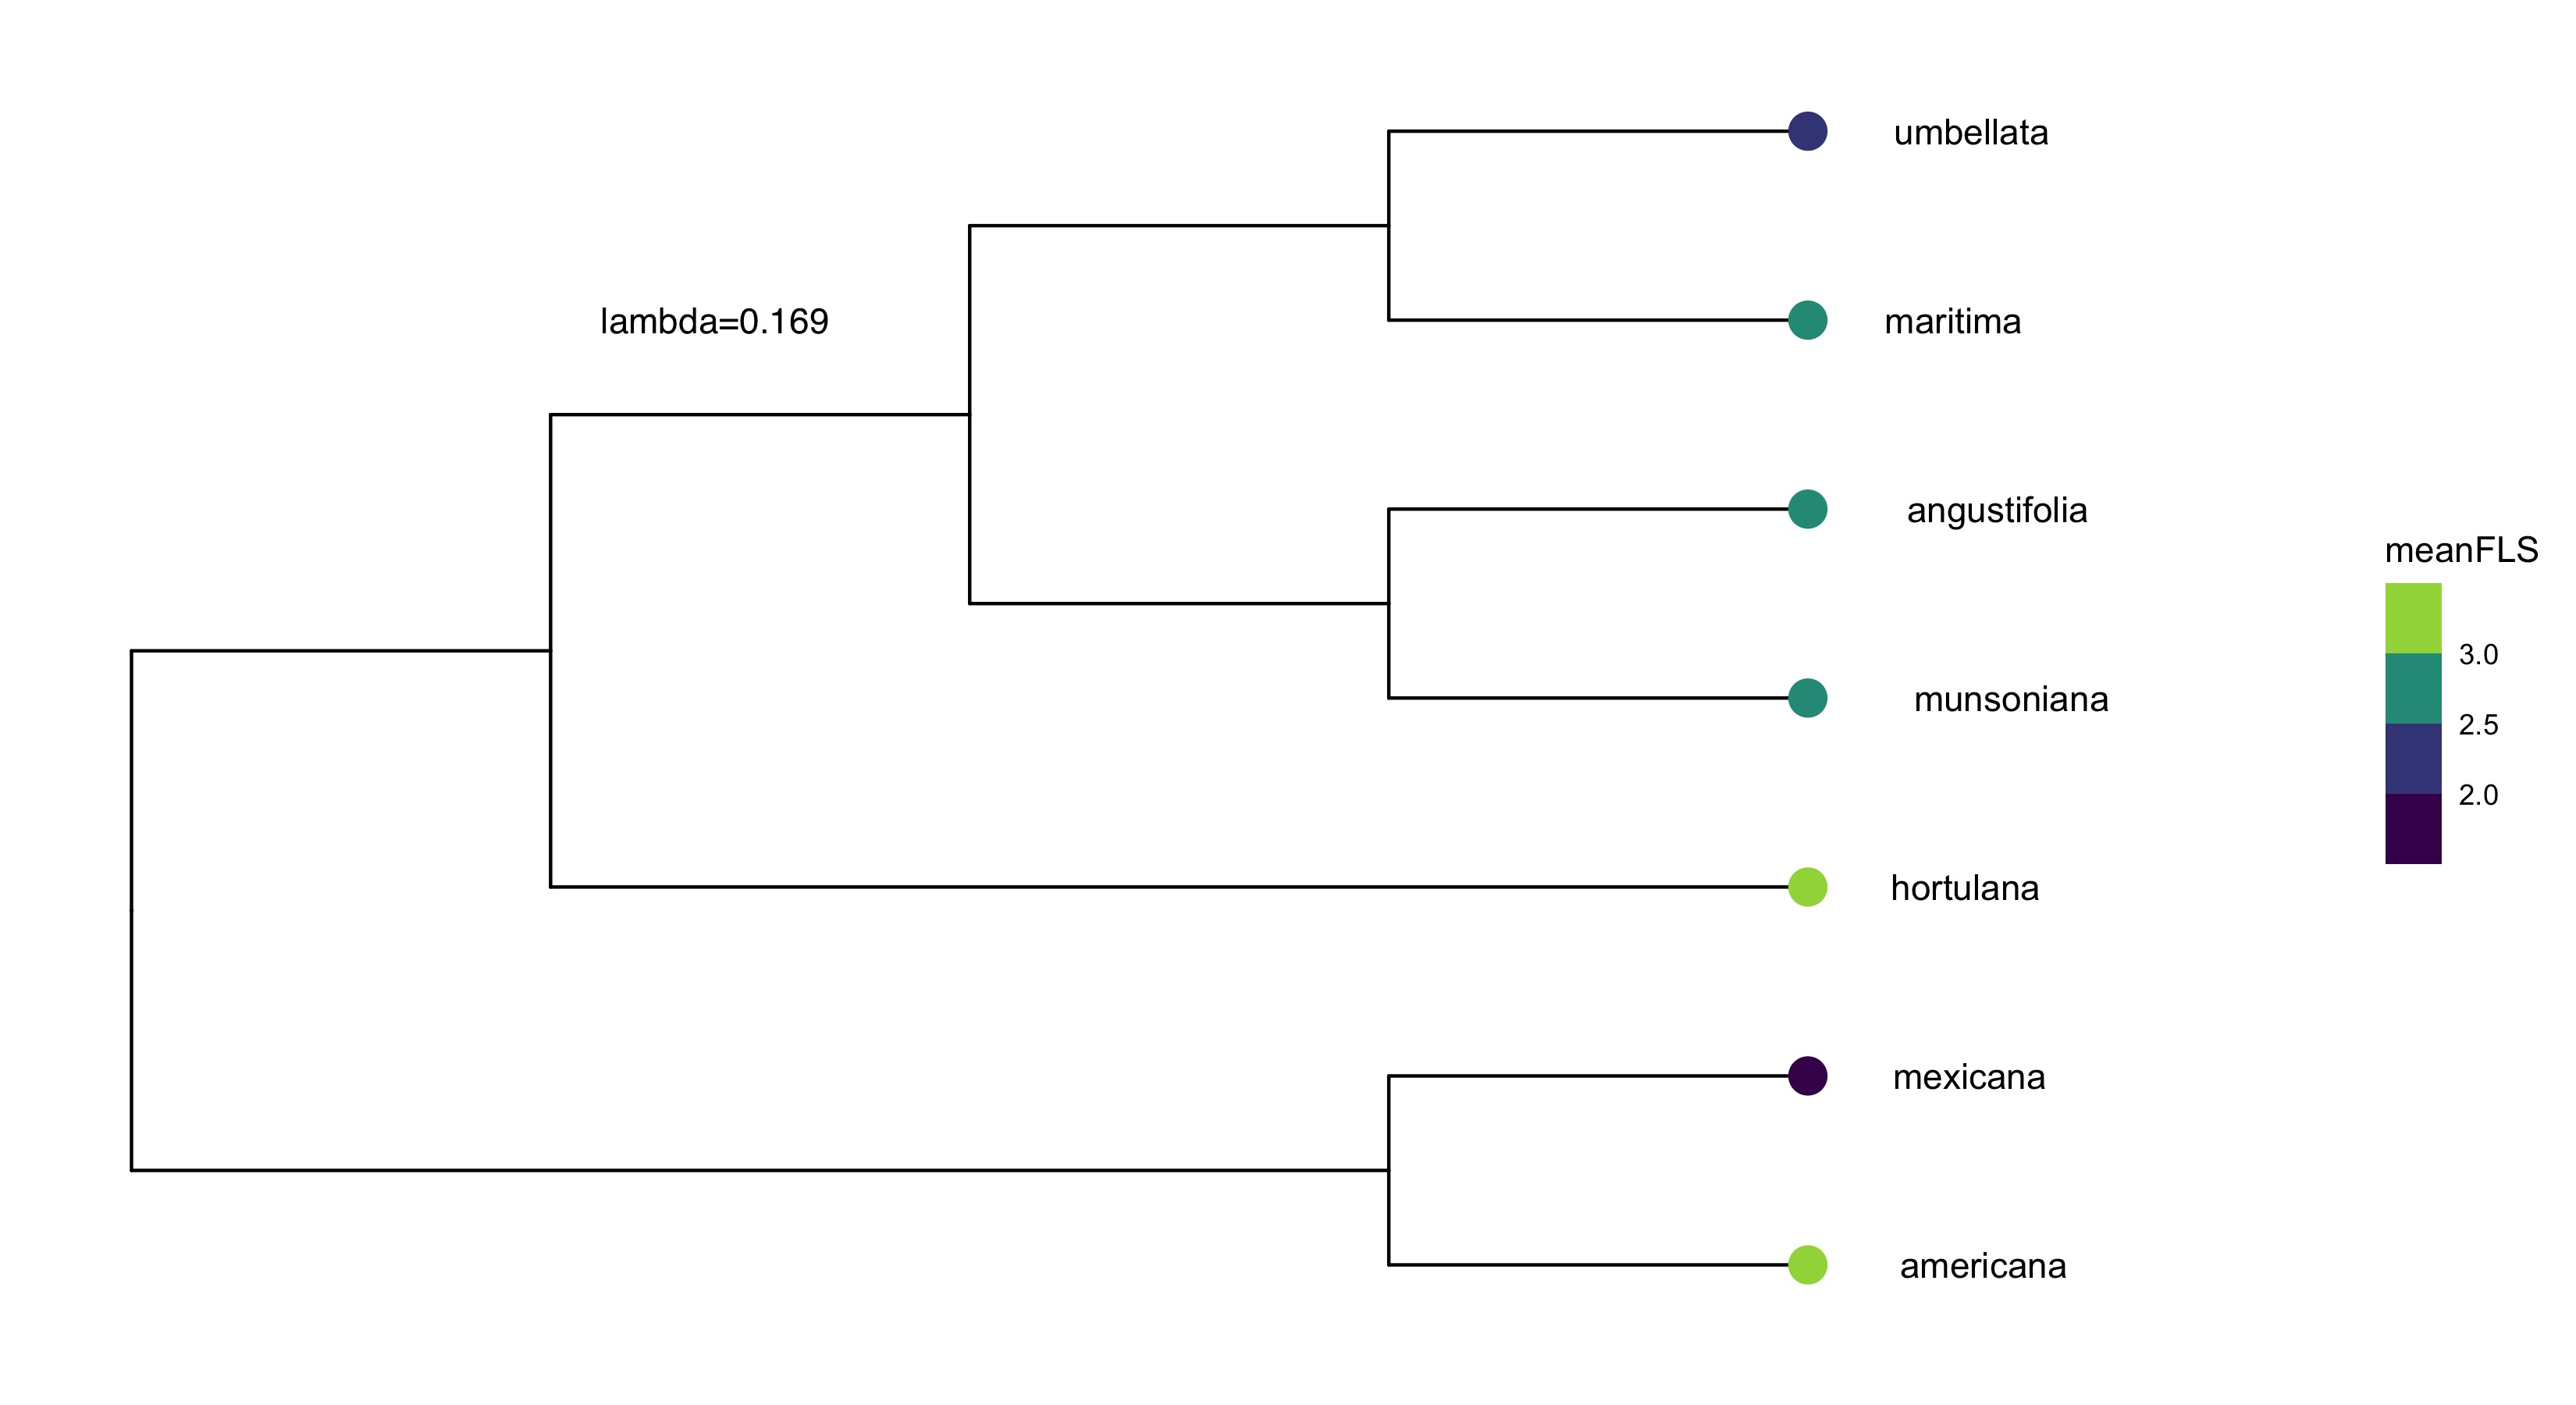
\includegraphics[width=\textwidth]{..//..//Plots/phylosig1.jpeg}
%    \caption{place holder for the phylgenies: Ideally will have all N.A. Prunus \texit{and} Prunocerasus }
%    \label{fig:phylo1}
%\end{figure}

\begin{figure}[h!]
    \centering
 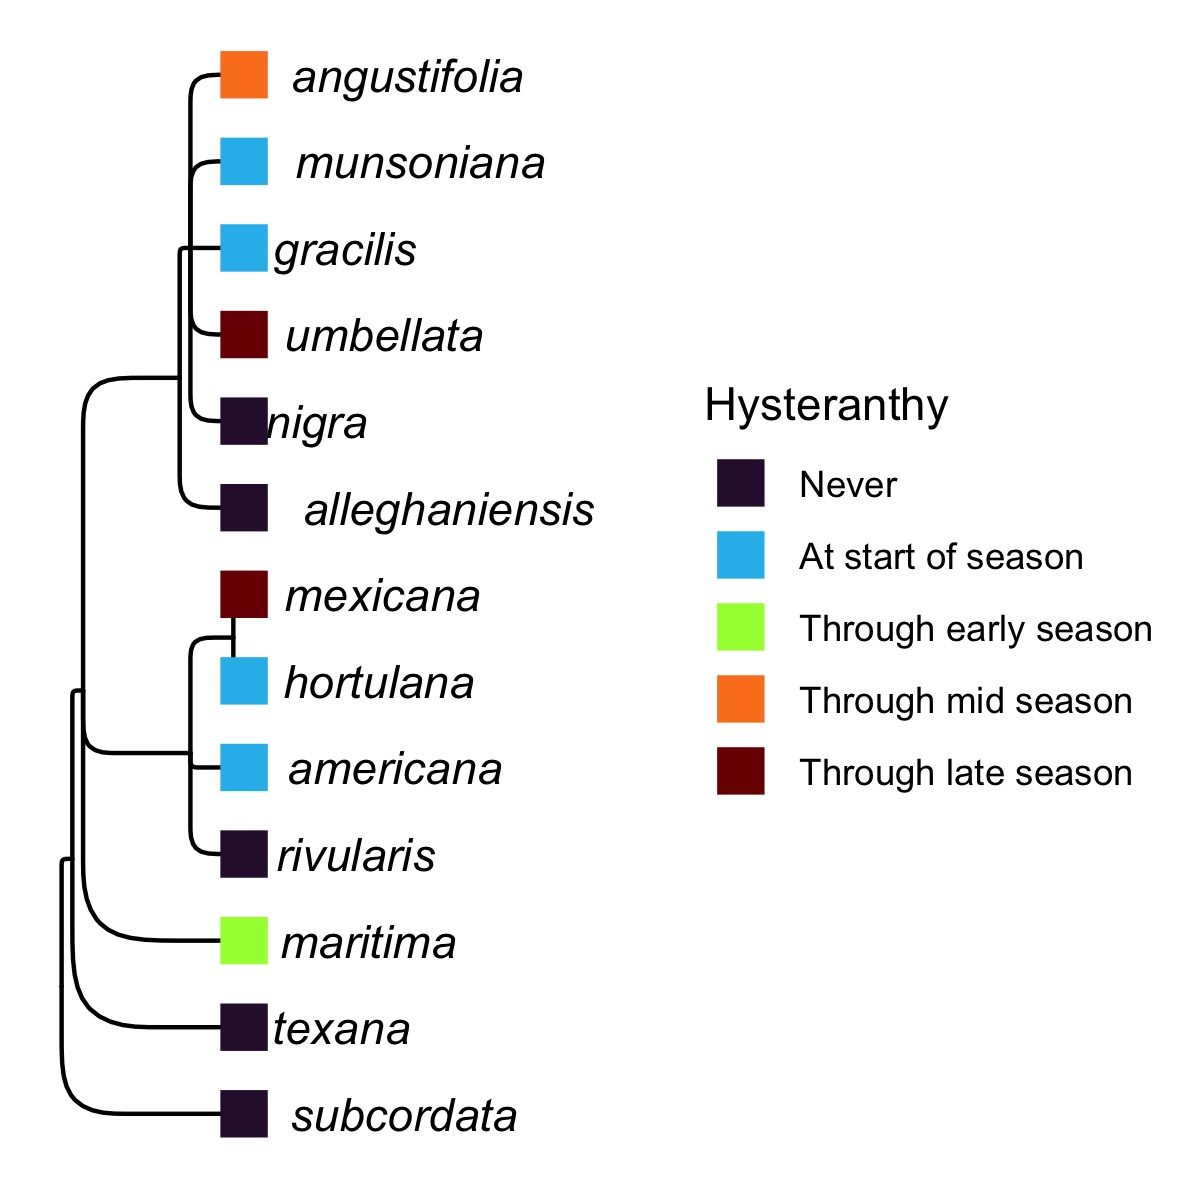
\includegraphics[width=.6\textwidth]{..//..//Plots/phylosig2.jpeg}
    \caption{place holder for the phylgenies: Ideally will have all N.A. Prunus \texit{and} Prunocerasus }
    \label{fig:phylo2}
\end{figure}

%\begin{figure}[h!]
 %   \centering
 %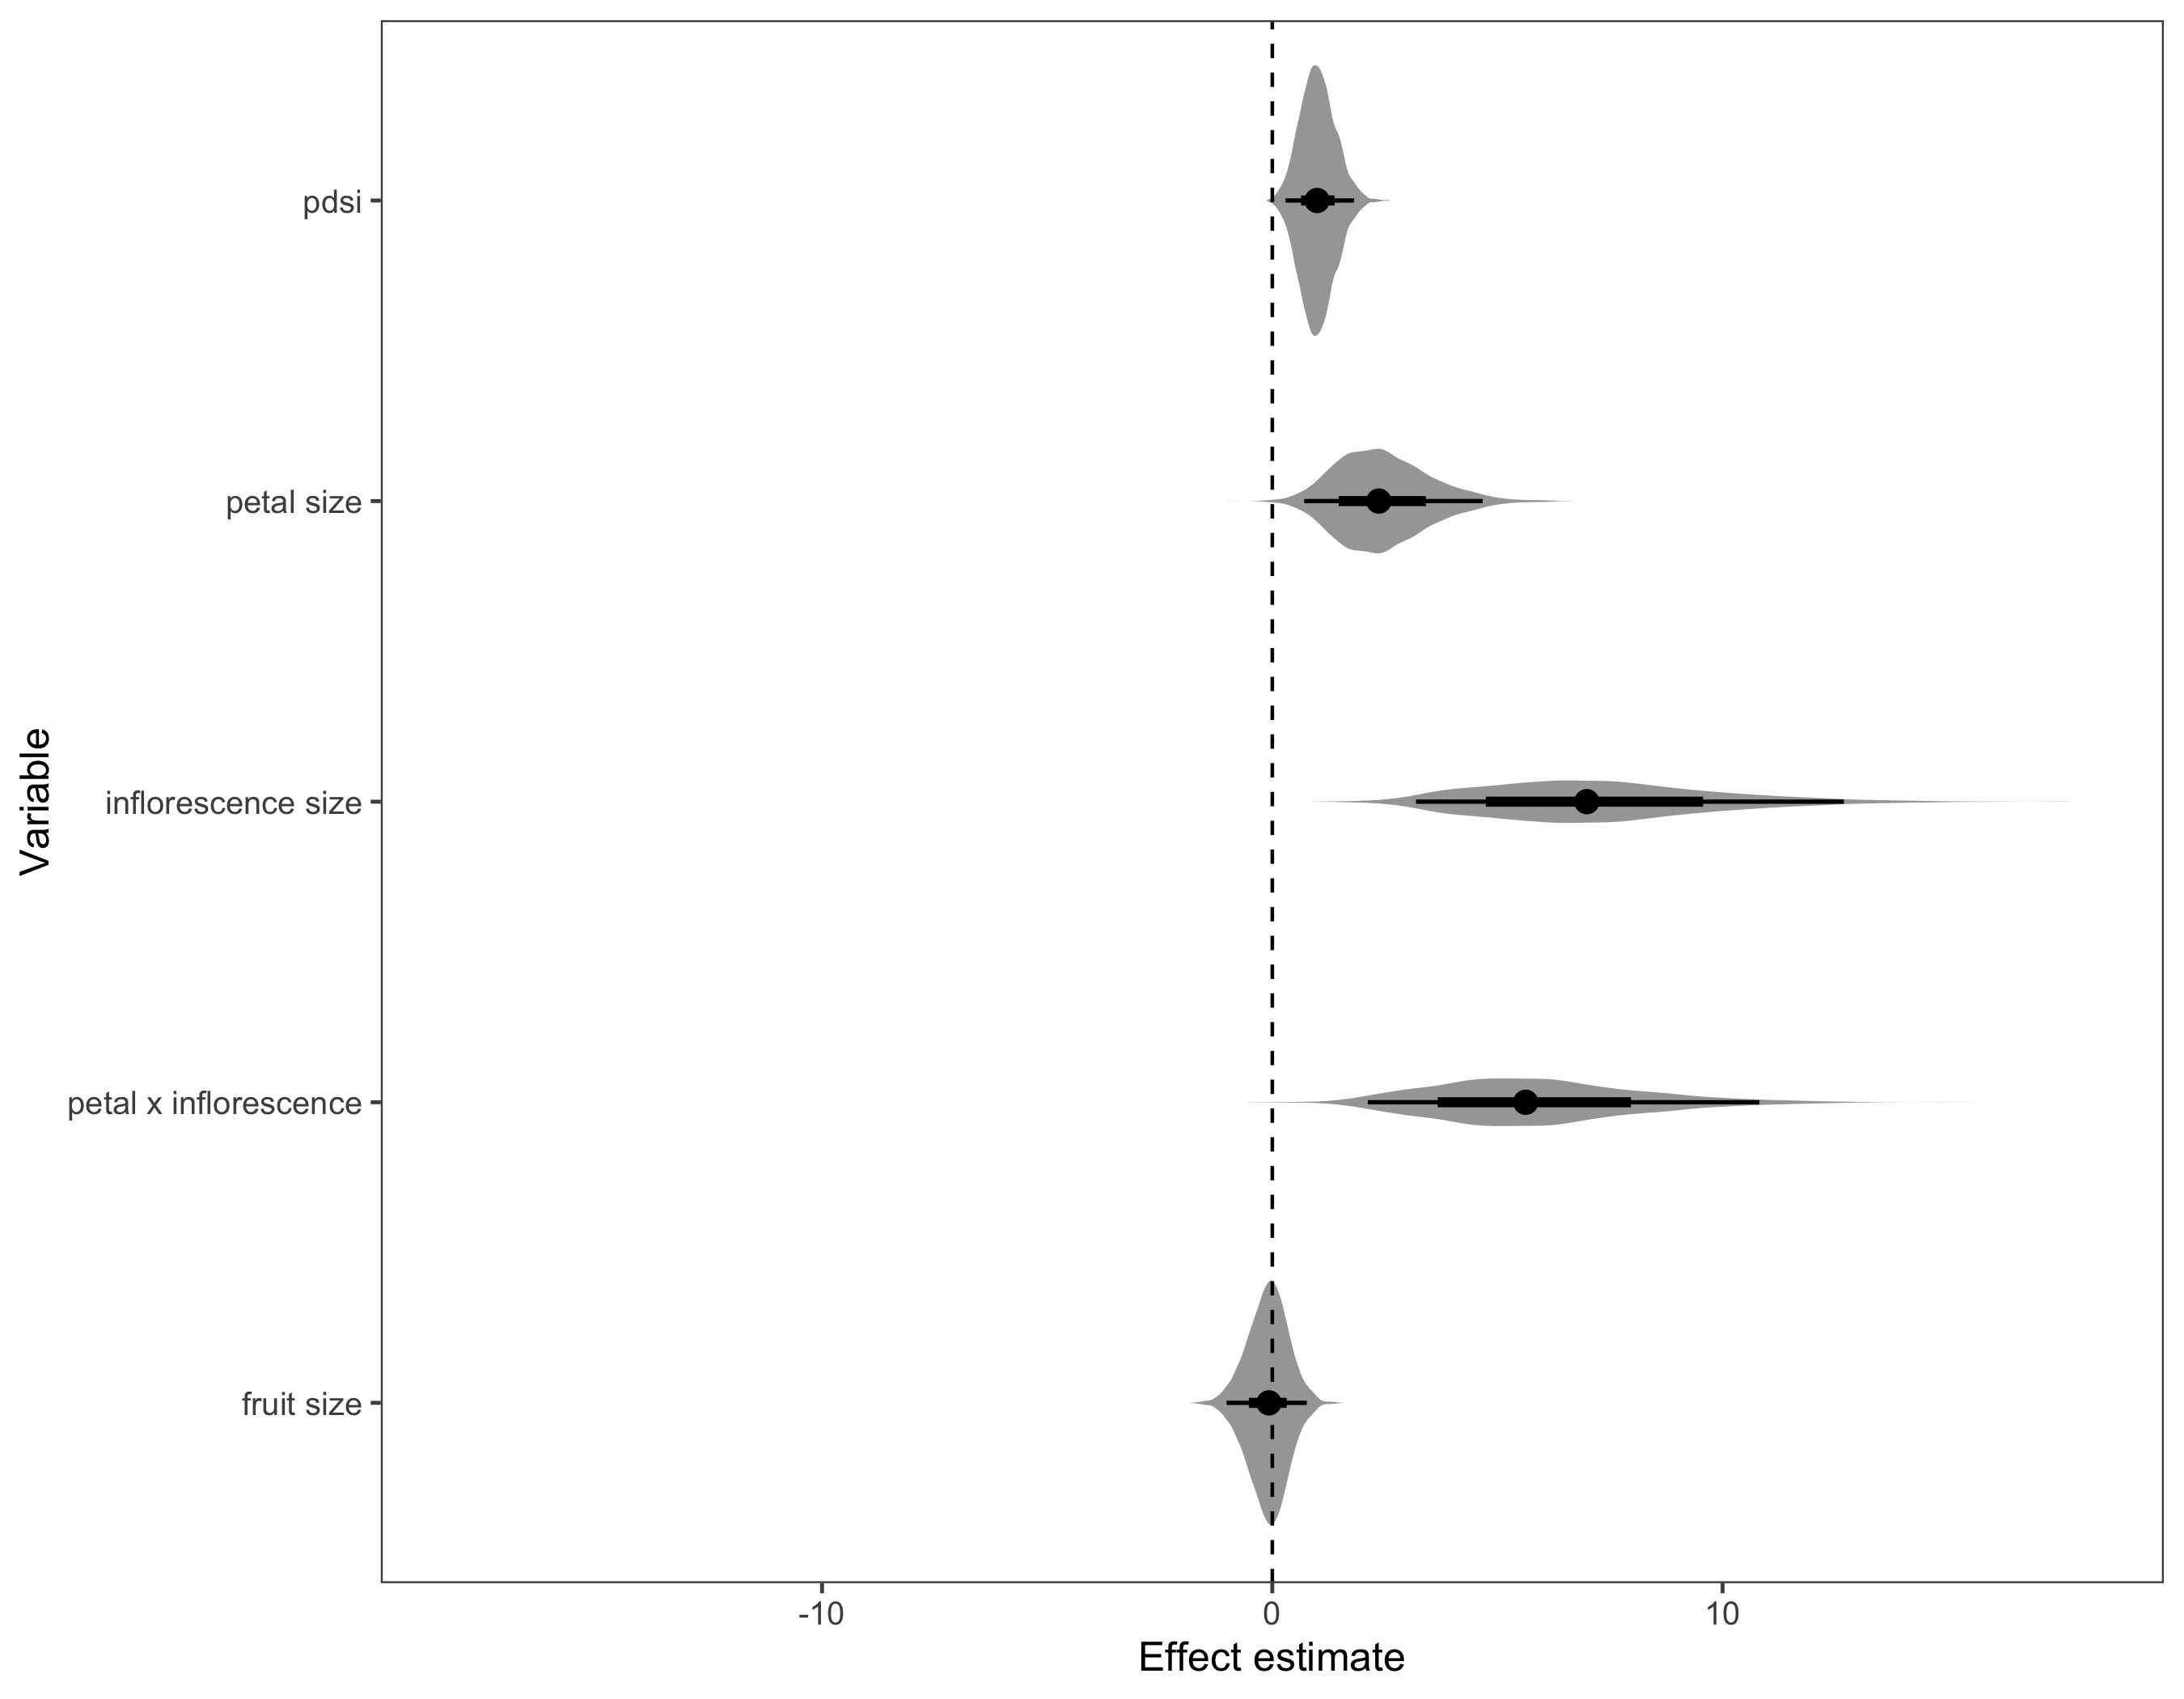
\includegraphics[width=\textwidth]{..//..//Plots/fullprunus_mus.jpeg}
 %   \caption{From the full genus analysis: Positive is less hysteranthus so aridity increases ihysteranthy, flower size decreases (ie smaller flowers- more hysteranthous) and no relationship with fruit size }
  %  \label{fig:cherries}
%\end{figure}



\begin{figure}[h!]
    \centering
 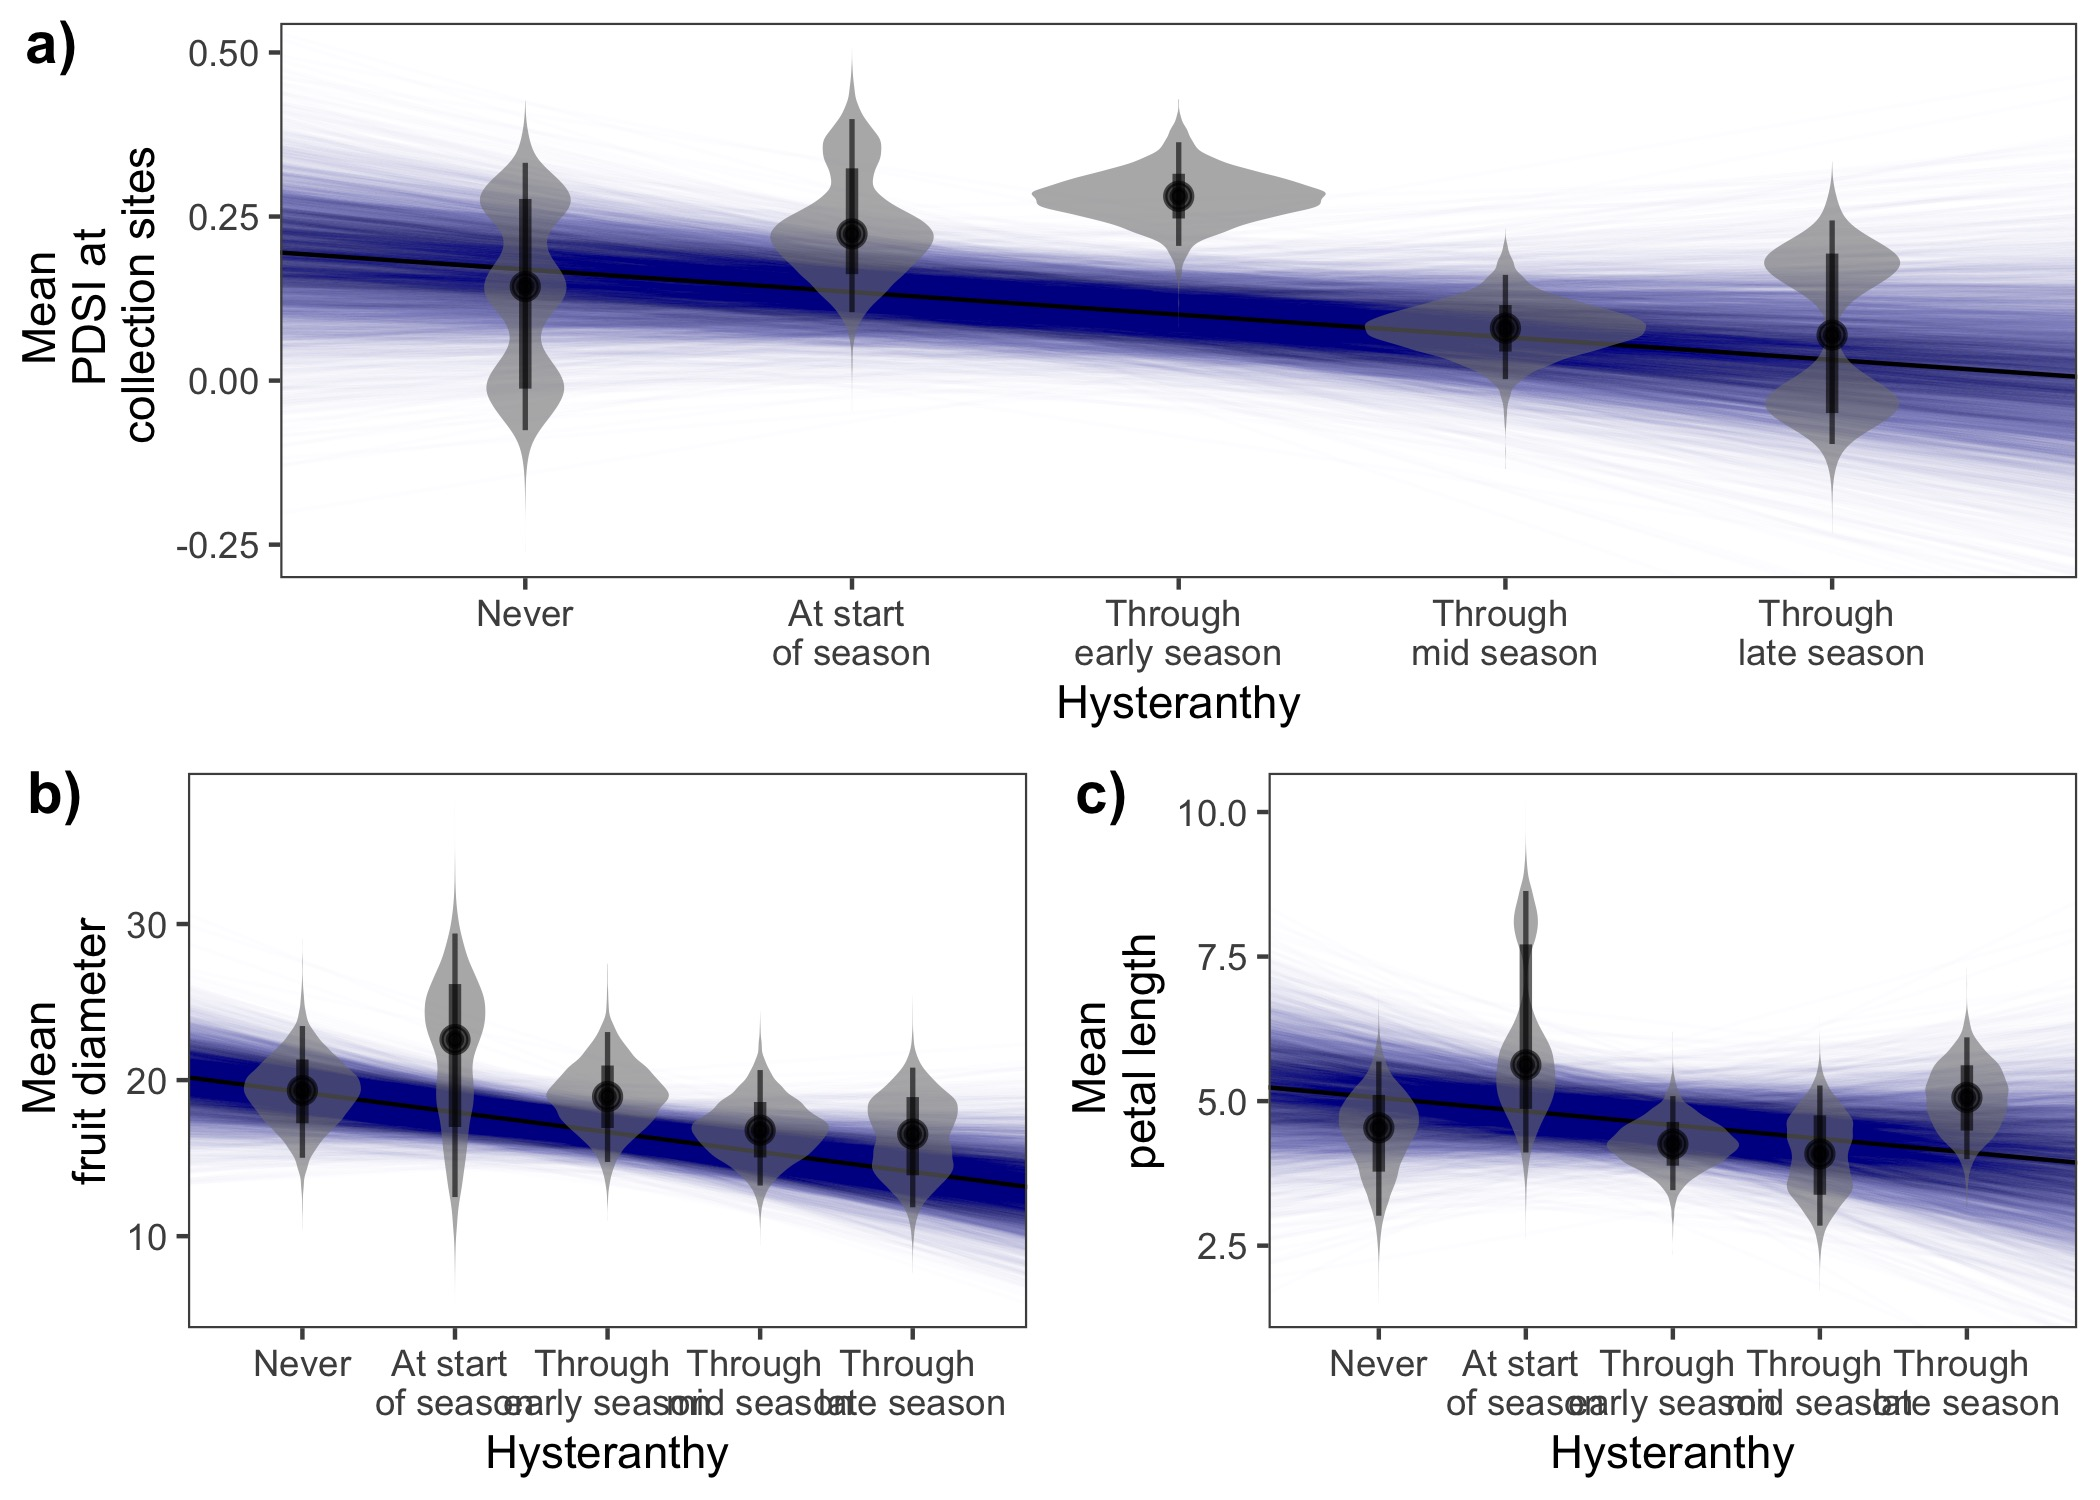
\includegraphics[width=\textwidth]{..//..//Plots/dataplots.jpeg}
    \caption{Relationships between the duration of hysteranthy across the flowering period and environmental and biological traits  } }
    \label{fig:prunes}
\end{figure}


%\begin{figure}[h!]
 %   \centering
 %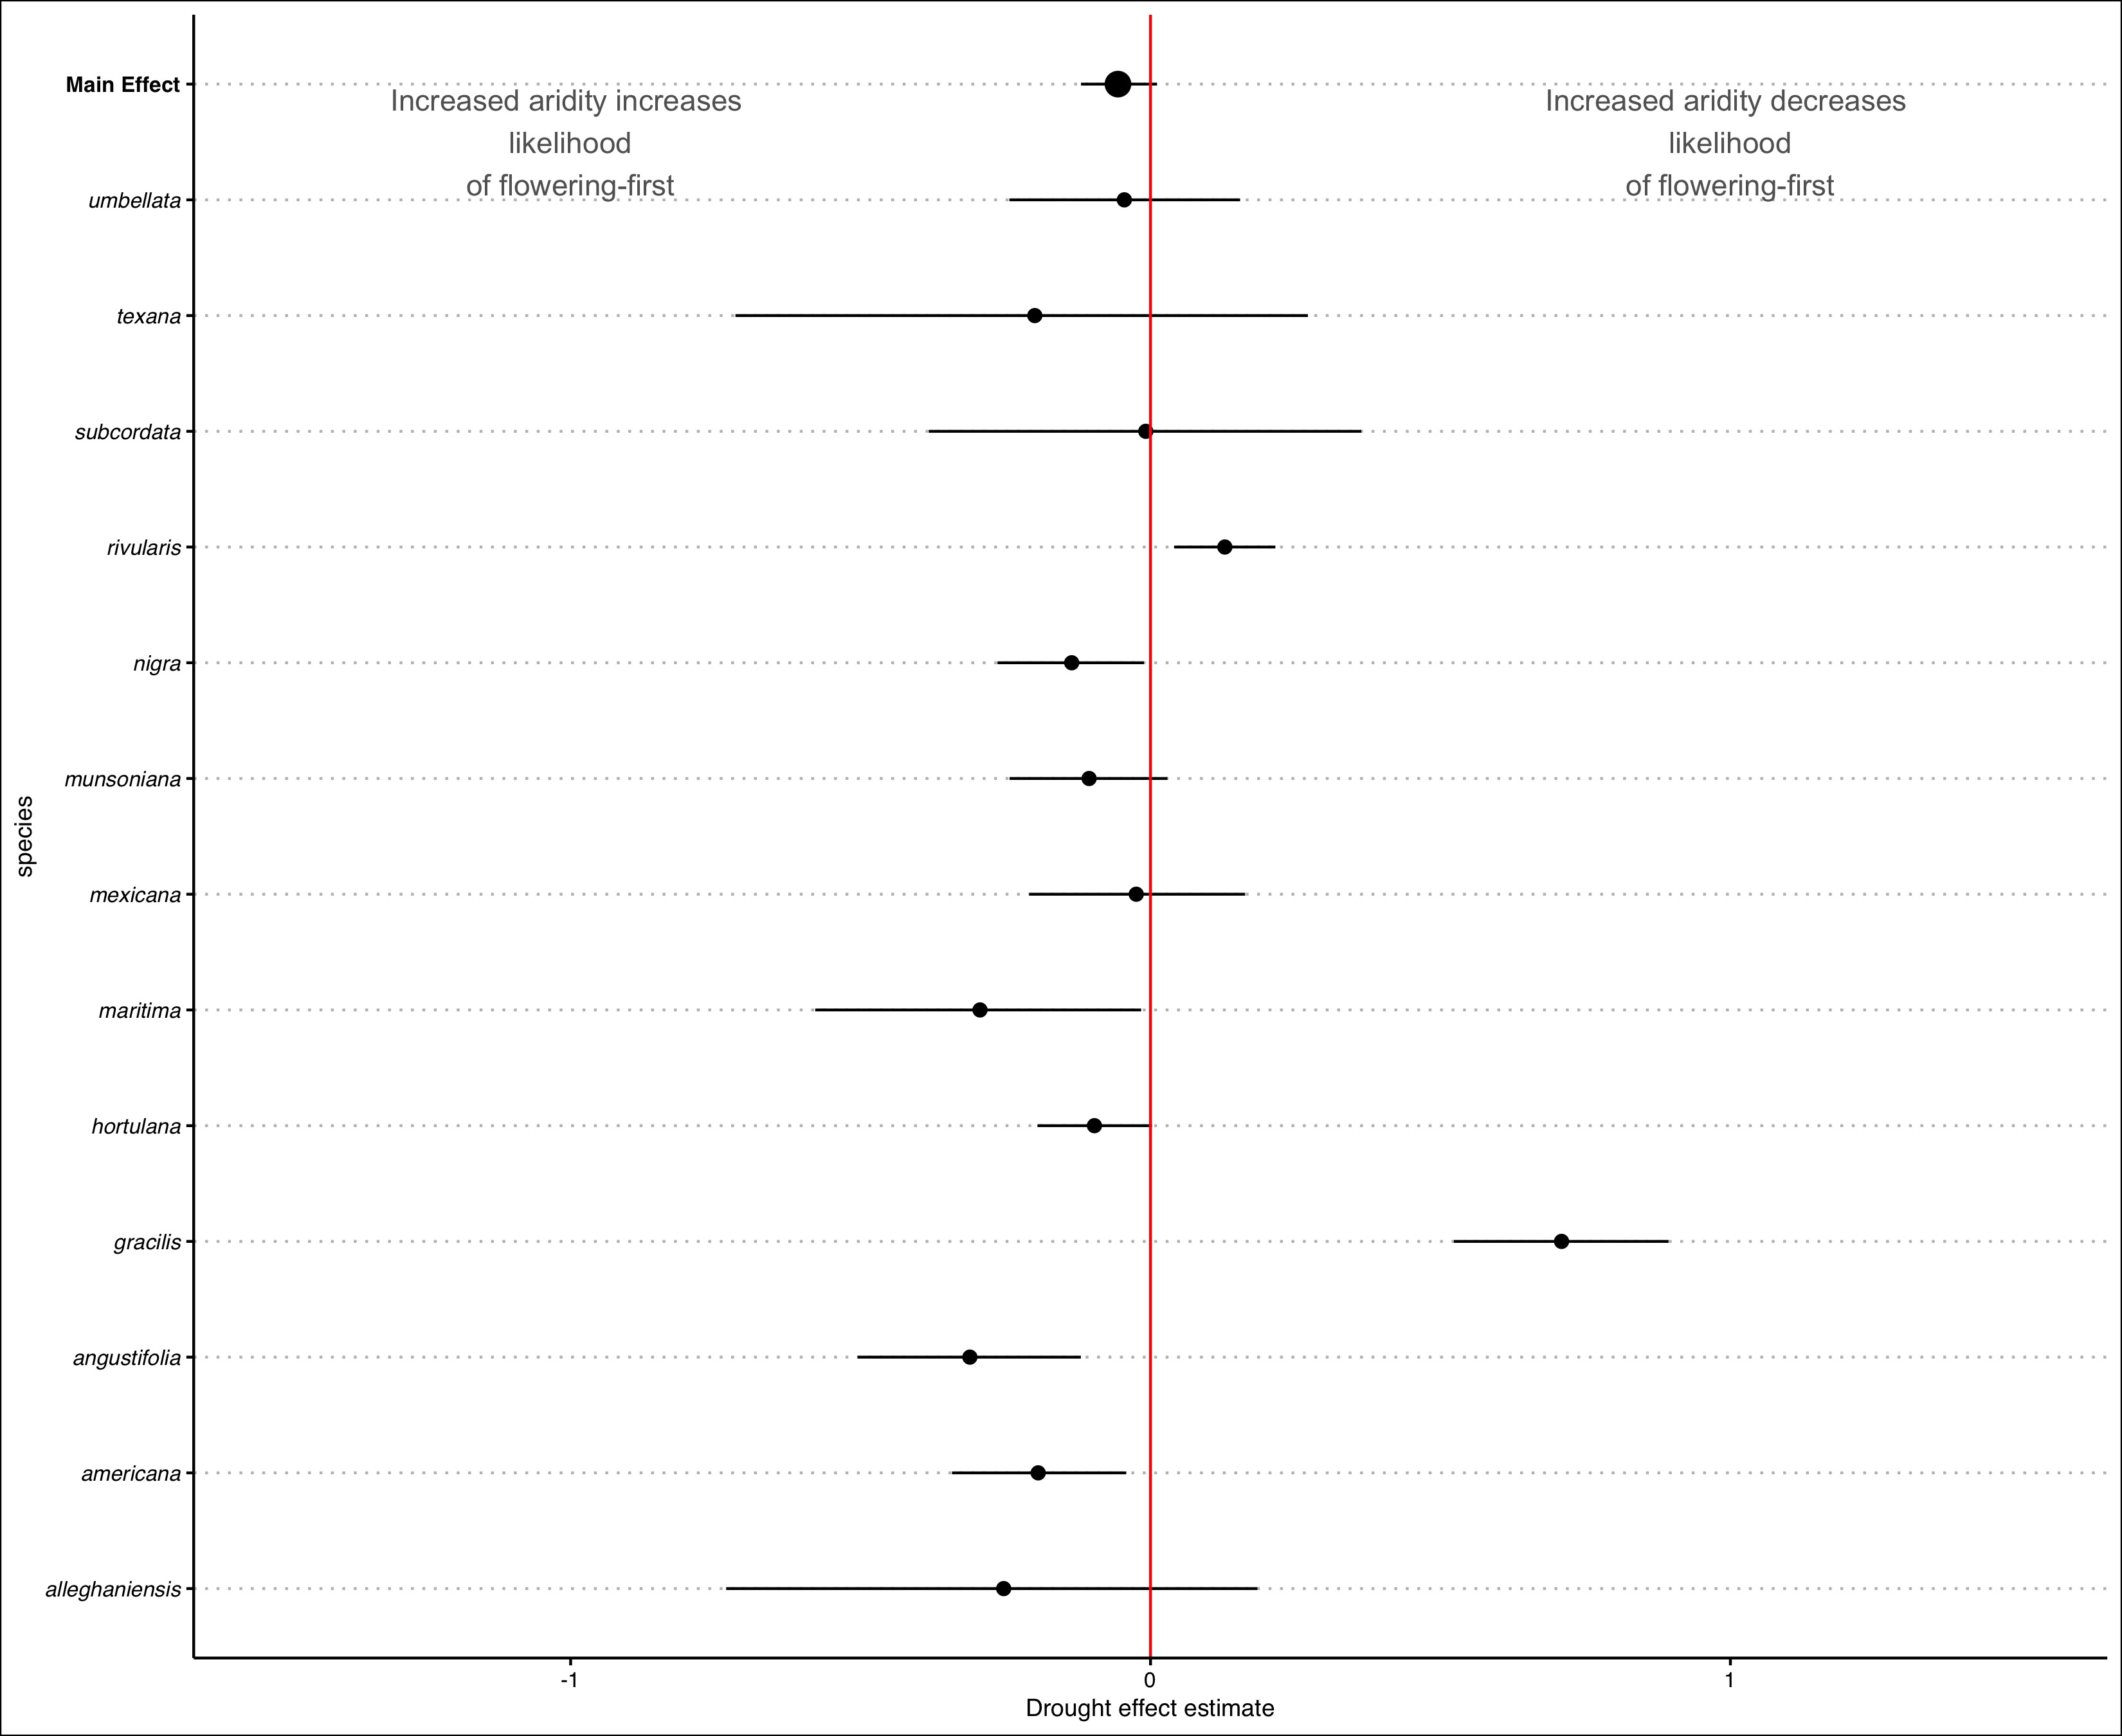
\includegraphics[width=\textwidth]{..//..//Plots/droughtstuff.jpg}
  %  \caption{Hysteranthy more likely in drought years.}
   % \label{fig:plastic}
%\end{figure}

\end{document}
